\begin{figure}[!ht]
    \centering
    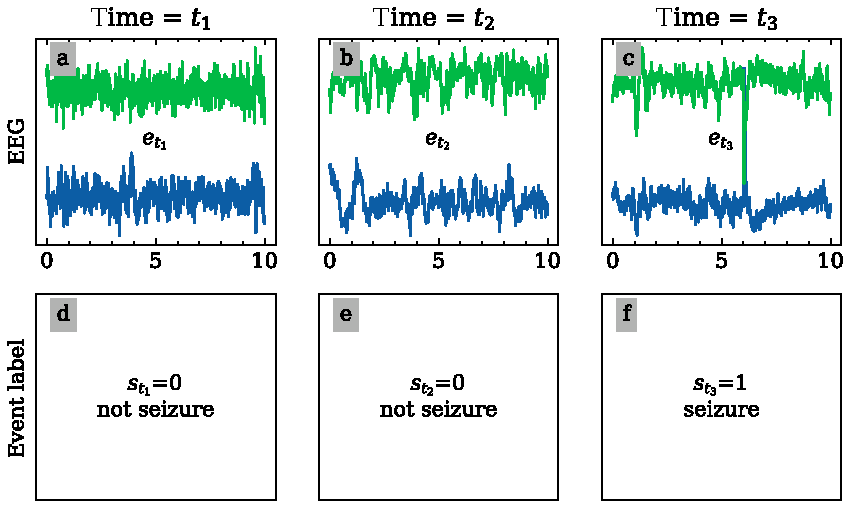
\includegraphics{c3Bsle/Figs/intro/sample_space.pdf}
    \Caption{Sample space $\Omega_E \times \Omega_S$}{In the probabilistic model, EEG segments and seizures are plausible events. For example, a 2-channel 400 $Hz$ EEG segment of length 10 seconds is a realization of the random variable E 
    supported by $\mathbb{R}^{2 \times 400}$. Likewise, the occurrence of a seizure at time $t_i$ is denoted by $s_{t_i} = 1$ as opposed to $s_{t_i} = 0$.}
    \label{fig:c3bsle:sample_space}
\end{figure}

